\paragraph{Creazione Questionario}

\label{Creazione questionario}

\begin{figure}[ht]
	\centering
	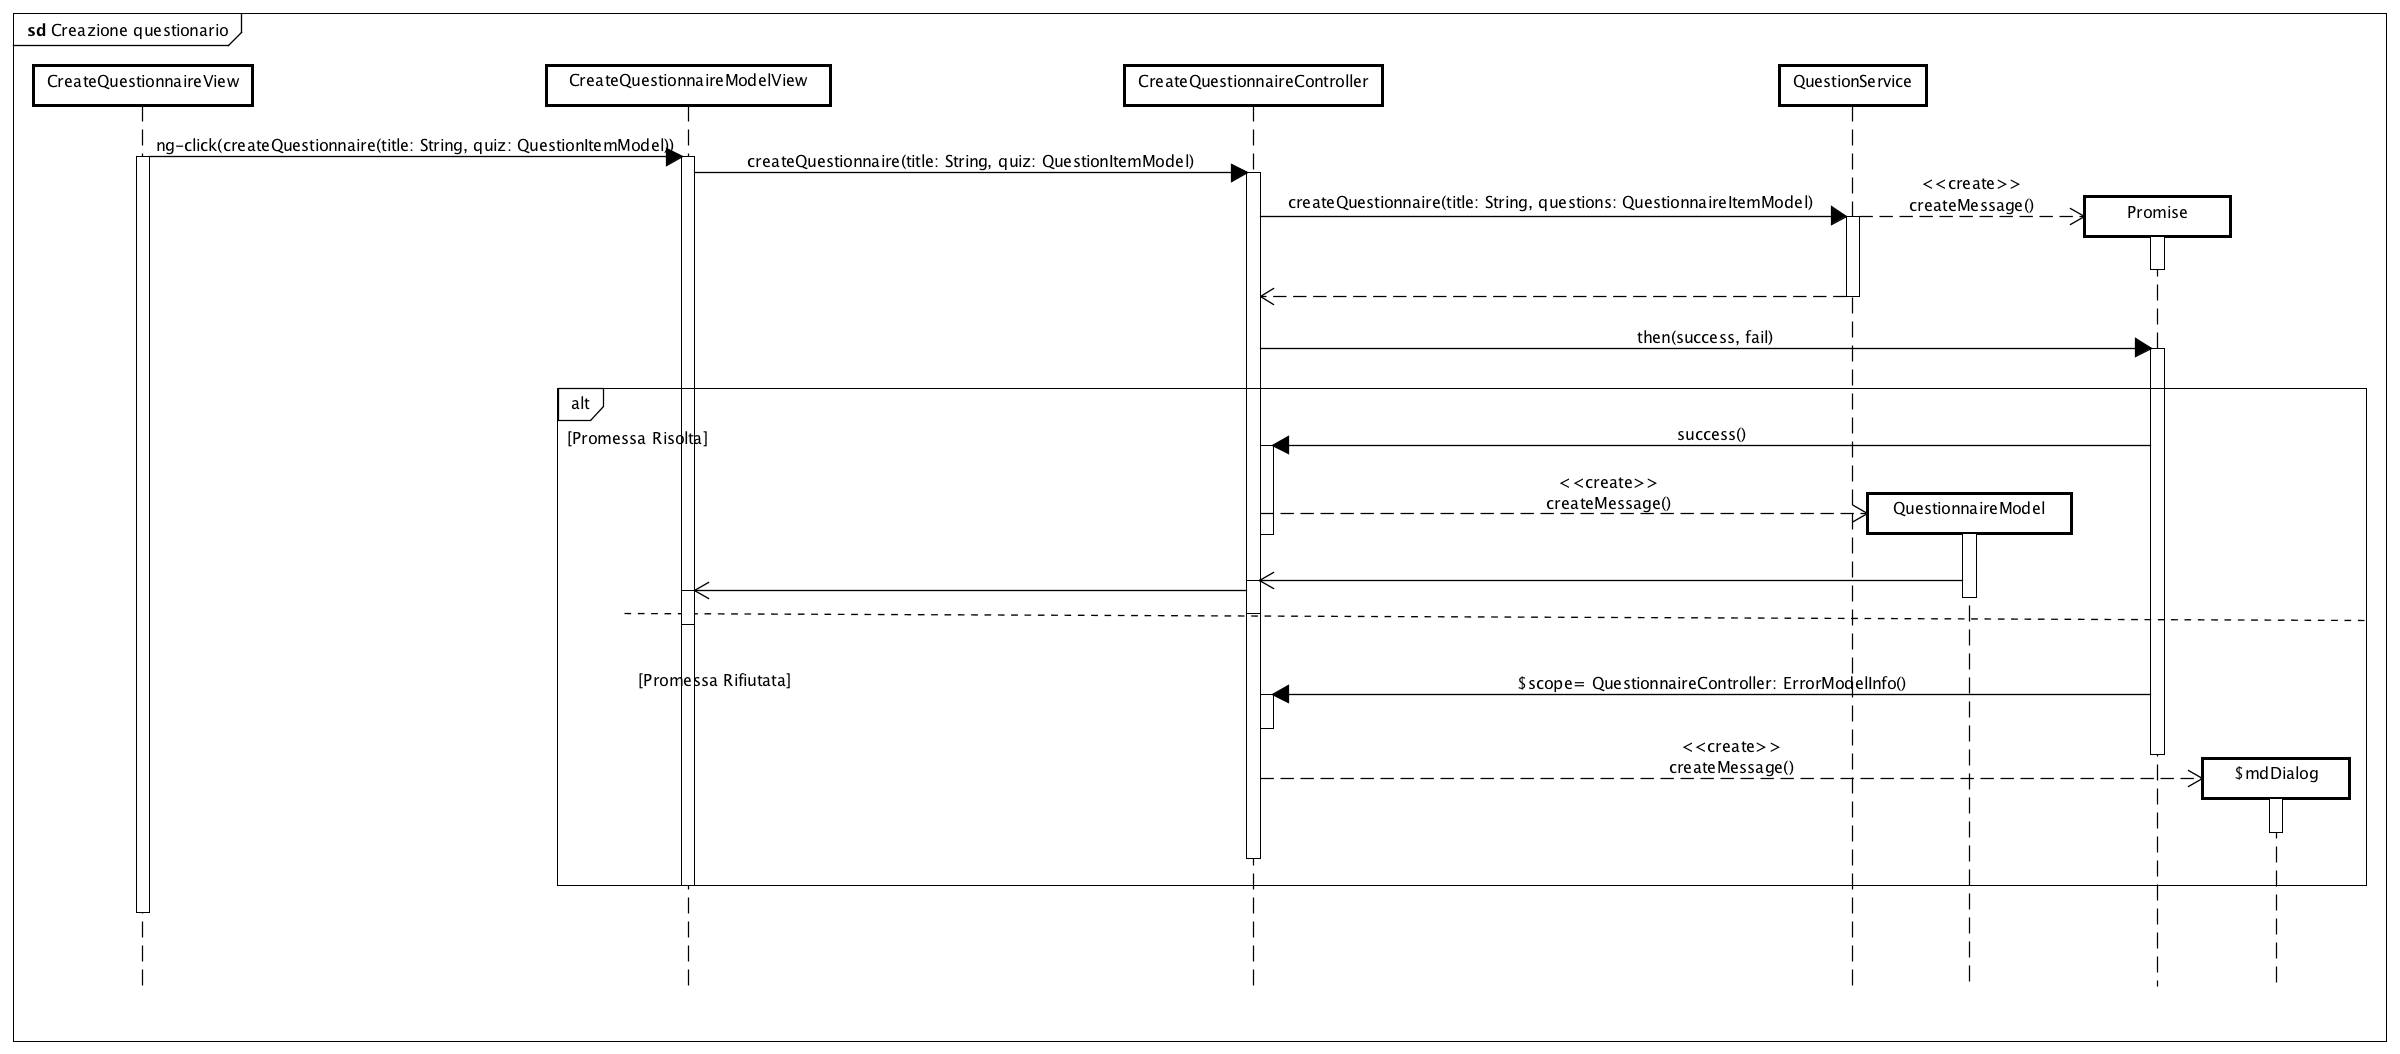
\includegraphics[scale=0.25,keepaspectratio]{UML/DiagrammiDiSequenza/Front-end/QuestionnaireCreation.png}
	\caption{Creazione questionario}
\end{figure} \FloatBarrier

Dopo che l'utente avrà selezionato il link di creazione questionario, verrà richiamato il metodo del controller che richiederà al service l'inserimento del questionario tramite chiamata a risorse del back-end. Se la promessa creata dal service verrà accettata il questionario sarà inserito, altrimenti verrà restituito un oggetto contenente il testo dell'errore. 